%*******************************************************************************
%Example chapter file for books, Copyright A K Peters, Ltd.
%*******************************************************************************
\chapter{Exploring Mobile vs. Desktop OpenGL Performance}{Jon McCaffrey}
\label{Exploring-Mobile-vs-Desktop-OpenGL-Performance}

\section{Introduction}

The stunning rise of mobile platforms has opened a new market for new 3D
applications and games where, excitingly, OpenGL ES is the \textit{lingua
franca} for graphics. However, mobile platforms and GPUs have performance
profiles and characteristics that may be unfamiliar to desktop developers.
Developers making the transition from desktop to mobile need to be aware of
the limits and capabilities of mobile devices to create the best experience
possible for the given hardware resources.  This chapter surveys mobile GPU
design decisions and constraints, then explores how these affect classic
rendering paradigms.

First, we examine how mobile and desktop GPUs differ in design goals, scale and
architecture.  We then look at memory bandwidth consumption, which greatly
affects performance and device power, and break it down into the contributions
of display, composition, blending, texture access, and anti-aliasing.  After
that, our focus shifts towards optimizing fragment shading with limited compute
power.  We look at ways to eliminate shading work entirely if we can or to
minimize it or render it more efficient if we can't.  

Finally, we discuss the relationship between vertex and fragment shaders and
how it is affected by different mobile GPU architectures, and end with some
tips for optimizing vertex data for efficient reads and updates.

\section{Important Differences and Constraints}\label{Jon-McCaffrey:Constraints-Inspire-Creativity}

\subsection{Differences in Scale}
\label{Jon-McCaffrey:Architectural-Differences} Modern mobile devices are
capable devices, but they face much greater limitations than desktop systems in
terms of cost, chip die size, power consumption, and heat dissipation.

Power consumption is a major concern for mobile platforms that is much less
pressing on desktop.  Mobile devices must run off batteries small enough to fit
in the body of the device, and a short battery life is frustrating and
inconvenient to the user.  Mobile hardware is built to use less power than
desktop hardware via lower clock frequencies, narrower busses, smaller chips,
smaller data formats, and by limiting redundant and speculative work.  Display
and network take a great deal of power, but OpenGL applications contribute to
power consumption, especially through computation and through off-chip memory
accesses.

Power consumption is doubly-impactful on mobile devices, since power consumed
by the processor, GPU, and memory is largely dissipated as heat.  Unlike
desktop systems with active air cooling, good air circulation, and large heat
sinks to radiate heat, mobile systems are usually passively cooled and have
contrained bodies with little room for large sinks or radiating fins.  Excess
heat generation is not only potentially damaging to components, it's also
noticeable and irritating to users of hand-held products.

Die size and cost are also greatly different between mobile and desktop.
High-end desktop GPUs are some of the largest mainstream chips made, with over
3 billion transistors on recent models \cite{Walton10}.  Both the large area
and the effect of area on yield mean increased cost.  A discrete GPU also means
a separate package and mounting, and the expected cost increase.  In mobile
systems however, the GPU is usually one component on an integrated
\textit{System on a Chip (SoC)} designed for mobile and embedded applications,
which means that a mobile GPU is a fraction of the cost and area of a desktop
GPU.

\subsection{Differences in Rendering Architecture}
\label{Jon-McCaffrey:differences-in-rendering-architecture}
\index{tiling} \index{Immediate-Mode Rendering} Mobile and desktop GPUs don't
differ only in scale.  Mobile GPUs such as the Imagination Tech SGX543MP2 used
in the Apple iPhone 4S/iPad 2 and the ARM Mali-400 used in the Samsung Galaxy S2
use a \textit{tile-based} rendering architecture \cite{Klug11a}.  In
contrast, desktop GPUs from NVIDIA and ATI and mobile GPUs like the
GeForce ULV GPU used in the Samsung Galaxy Tab 10.1 use \textit{Immediate Mode
Rendering (IMR)}.

In IMRs, vertices are transformed once and primitives are rasterized
essentially in order.  If a fragment passes depth-testing (assuming the
platform has early-z), it will be shaded and will write to the framebuffer.
However, a later fragment may over-write this pixel, nullifying the earlier
work done and writing the framebuffer again.  This behavior is known as overdraw.
Even without overdraw, the depth buffer still must be read for later fragments 
generated at a pixel location in order to reject them.

\begin{figure}[h!]
    \caption{IMRs render each primitive only once, and render the entire framebuffer in a single pass}
    \centering
        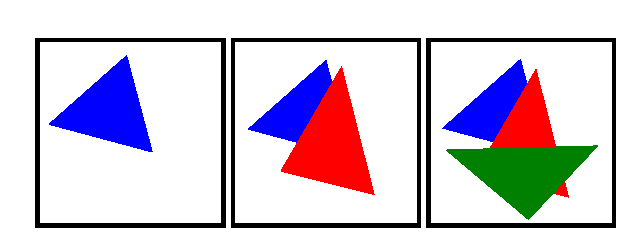
\includegraphics{mccaffreyFigs/IMR.eps}
\end{figure}

Tilers instead divide the framebuffer into tiles of pixels.  All draw
commands
 are buffered.  At the end of the frame, for each tile, all
geometry for the scene is re-rendered and rasterized into a framebuffer cache
with that tile scissored out.  Once all pixels have been resolved, the entire
tile is written out to memory.  This saves redundant framebuffer writes and
allows for fast depth-buffer access, since depth-testing and depth writes can
be performed with the local framebuffer cache.  The end goal is to limit the
memory bandwidth consumed by color and depth buffer access.

\begin{figure}[h!]
    \caption{Tiling architectures divide the scene into tiles, and render all primitives into each tile using a fast framebuffer cache.}
    \centering
        
\includegraphics{mccaffreyFigs/tiling.eps}
\end{figure}

Tiling doesn't come for free.  The scene geometry must be re-transformed and
clipped for each
 tile, so to maintain a balanced pipeline additional vertex
processing power is
 needed.  Bandwidth will also be spent re-reading vertex
data for each tile.  The digital
 logic for tiling, repeated vertex shading,
and a fast framebuffer cache also
 takes transistors from raw fragment shading
horsepower.  Tiling also requires buffering commands deeply, leading to a more
complicated hardware and driver implementation, and the fact that the rendering
of each primitive cannot be neatly placed in single interval of time makes
performance analysis more difficult.  For more tips on
 performance tuning
specific to tiling architectures, see \textit{Performance
 Tuning for
Tile-Based Architectures} \cite{Chapter TODO}
 

\index{Tile-Based Deferred Rendering} There is an additional group of tilers
which use \textit{Tile-Based Deferred Rendering (TBDR)}, like the Imagination Tech SGX
family.  The idea is to rasterize all primitives in a tile before performing
any fragment shading.  This allows \textit{Hidden Surface Removal (HSR)} and
depth-testing to be performed in a fast framebuffer cache before any fragment
shading work is done.  Assuming opaque geometry, each pixel is then shaded and
written to the framebuffer exactly once.

Architecturally, the mobile GPU landscape is not homogenous.  Optimizations may
affect the different architectures very differently, so it is important to test
on multiple devices for cross-platform releases.  \subsection{Differences in
Memory
Architecture}\label{Jon-McCaffrey:differences-in-memory-architecture}

On desktop systems, middle-to-high-end GPUs are discrete devices which
communicate with the rest of the system via a peripheral bus like
\textit{PCIe}, althought some desktop CPUs are now shipping with capable
integrated GPUs, like the AMD Llano processors.  For good performance, this
means that GPUs must include their own dedicated memory, since accessing system
memory through a peripheral bus for all memory accesses would be too slow in
terms of bandwidth and latency.  While this increases cost, it is an
optimization opportunity since this memory and its configuration, controller,
caching, and geometry can be optimized for graphics workloads.

For example, the NVIDIA \textit{Fermi} architecture uses GDDR5 memory that is
heavily partitioned \cite{Walton10} to allow for a wide memory interface.
There are no other components competing for this bandwidth, since except for
uploads from the rest of the system and scan-out for output devices, the GPU is
the only user of this memory.

\index{System-on-a-Chip} \index{Unified Memory Architecture}

In mobile devices, on the other hand, the GPU is usually integrated into the
same SoC as the CPU and other components.  To save cost, power, die size, and
package complexity, the GPU shares the RAM and memory interface with the other
components.  This is known as an \textit{Unified Memory Architecture (UMA)}.  A
common memory type is the low-power LPDDR2, which has a 32-bit wide
interface \cite{Klug11b}.  Not only is this memory general-purpose, the GPU now
shares bandwidth with other parts of the system like the CPU, network, camera,
multimedia, and display, leaving less dedicated bandwidth available for
rendering and composition.

\index{bandwidth}

There are some performance advantages to a unified memory architecture, besides
the savings in cost and complexity.  With discrete GPU's the peripheral bus
could become a bottleneck for transfers, especially for non-PCIe buses with
asymmetric speeds \cite{Elhasson05}.  With a UMA, OpenGL client and server data
are in fact stored in the same RAM.  Even when it is not possible to directly
access server-side data with \texttt{glMapBufferOES}, there are fewer
performance cliffs lurking in transfers between OpenGL client and server data,
and using client-side data for dynamic vertices or indices may not have as
great a performance penalty.  Data transfer and command latencies from the GPU to the
CPU are also likely to be lessened.

\index{Pixel Buffer Object}

One current limitation is that OpenGL ES does not yet have an extension for
\textit{Pixel Buffer Objects (PBO)}, meaning that pixel and texture data must
be transferred synchronously.  This makes the comparatively cheap bandwidth
between client and server data less useful, and also makes streaming assets
during run-time more difficult.

\section{Reducing Memory
Bandwidth}\label{Jon-McCaffrey:Reducing-Memory-Bandwidth}

\index{bandwidth}

Memory bandwidth pressure is one of the major performance pressures on mobile
devices, especially on games and other applications which also perform heavy
amounts of CPU-side work during the frame, or in multimedia applications which
have additional bandwidth clients besides the GPU and display.

Besides limiting performance, memory accesses external to the GPU consume a
great deal of power, sometimes more than the computation itself.
\cite{Antochi04}.

\begin{table}[htb]\centering \begin{tabular}{|c||c|c|} 
\hline \small{Device} & \small{CPU Write Bandwidth} & \small{GPU Write Bandwidth}   \\ \hline 
\hline \small{Motorola Xoom} & \small{2.6GBps} & \small{1.252GBps} \\ 
\hline \small{Motorola Droid X} & \small{1.4GBps} & \small{6.8GBps} \\ 
\hline \small{LG Thunderbolt} & \small{0.866GBps} & \small{0.518GBps} \\ 
\hline \small{Dell Inspiron 520} & \small{4.8GBps} & \small{3.8GBps} \\ 
\hline \small{Desktop System} & \small{14.2GBps} & \small{25.7GBps}\\
\hline
\end{tabular} 
\caption{Write bandwidth for CPU and GPU on different devices.  CPU write
bandwidth estimated by \textit{memset}.  GPU bandwidth estimated by glClear
followed by glFinish.  Desktop system has an Intel Core 2 Quad and NVIDIA
GeForce 8800 GTS.  The desktop system has significantly more bandwidth
available to the GPU than to the CPU, and CPU and GPU memory accesses do not
interfere with each other.}
\label{JonMcCaffrey:bandwidth} \end{table}

\subsection{Relative Display Sizes}\label{Jon-McCaffrey:relative-display-sizes}

\index{resolution} \index{display}

Despite the tight power and cost constraints for mobile devices, the display
resolutions of modern mobile devices are a considerable fraction of the
resolutions of desktop displays.  Even though the displays sizes are smaller,
mobile devices often have a higher pixel density to be viewable at a close
distance.

\begin{table}[htb]\centering \begin{tabular}{|c||c|c|c|} 
\hline \small{Device} & \small{Resolution} & \small{\% of 1280x1024 (20 in. monitory)} & \small{\% of 1920x1080 (24 in. monitor)}  \\ \hline 
\hline \small{Motorola XOOM} & \small{1280x800} & \small{\%78.13} & \small{\%49.38}\\ 
\hline \small{Apple iPad 2} & \small{1024x768} & \small{\%58.63} & \small{\%37.06}\\ 
\hline \small{Apple iPhone 4S} & \small{960x640} & \small{\%46.89} & \small{\%29.63}\\
\hline \small{Samsung Galaxy S2} & \small{800x480} & \small{\%30.00} & \small{\%18.52}\\ \hline
\end{tabular} 
\caption{Resolution comparison of desktop and mobile panels} 
\label{JonMcCaffrey:resolutions} \end{table}

\index{fragment shading}

With the limited fragment shading throughput and memory bandwidth of mobile
devices, these comparatively large display sizes mean that fragment shading and
full-screen or large-quad operations can easily become a bottleneck, since
these requirements scale proportionally with the number of output pixels.
Memory bandwidth is also a major power drain, making limiting bandwidth doubly
important.  Common large-quad operations include post-processing effects and user-interface composition.

Within mobile devices, there is also a large spread of resolution sizes
, especially between tablets and phone form factors, so testing
on multiple devices is important, for performance testing as well as
application useabilty.

\subsection{Framebuffer Bandwidth}\label{Jon-McCaffrey-Framebuffer-Bandwidth}

Basic rendering can consume surprisingly significant amounts of memory
bandwidth.  Assume the framebuffer has 16-bit color with 16-bit depth
\cite{Google11} and a 1024x768 resolution.  Accessing every pixel in the
framebuffer 60 times a second takes 94MBps of bandwidth.  So to write all the
pixels' colors every frame, at 60 frames a second, with 0\%
overdraw, takes 94MBps of bandwidth.

\index{bandwidth} \index{depth}

However, assuming an IMR architecture, to be able to render a scene, we also
usually perform a depth-buffer read for each rendered pixel.  Both the
depth-buffer and the color buffer are also usually cleared each frame.  And
when applications write to the color buffer while rendering the scene, they
also generally write the fragment depth to the depth-buffer.

The memory bandwidth consumption of the final framebuffer doesn't end when the
application is done writing it either.  After \texttt{eglSwapBuffers}, it may
need to be composited by the platform-specific windowing system, and then
scanned out to the display.  Unlike desktop systems which often have
dedicated graphics or framebuffer memory, this will also consume system memory
bandwidth.  This will consume an 94MBps of bandwidth just for
scanout, or at least 288MBps with composition(read, write to
composited framebuffer, and scan-out).

\index{composition}

 Thus with a depth and color clear, one depth buffer read, a depth and color
 buffer write, and display scanout, basic clear-fill-and-display operation
 consumes 564-752MBps of bandwidth, so even simple use cases consume a
 significant amount of memory bandwidth; anything interesting the application
 does only costs more bandwidth. If a 32-bit framebuffer is used, this number
 will be even greater.  This can be a significant portion of the bandwidth available on a mobile device, see \ref{JonMcCaffrey:bandwidth} for bandwidth
 measurements for some devices.
 %* TODO come up with better BW comparison *%

 Tile-based architectures can consume less bandwidth for this basic operation
 since they ideally handle the depth and color clears and the depth buffer
 reads within the framebuffer cache.  Use of the
 EXT\_discard\_framebuffer\cite{EXT_discard_framebuffer} extension saves
 additional bandwidth because it means the calculated depth buffer never needs
 to be written back to external memory from the framebuffer cache once the
 frame is complete. So a tile-based architecture will consume at least 188-377
 MBps for basic clear-fill-and-display operation.

\index{color depth}

Applications using a 32-bit framebuffer that may be bandwidth-bound should
experiment with a lower-precision format.  Since the output framebuffer is not
often used in subsequent calculations, the loss of numerical precision is not
propagated and magnified.  One valid concern is banding or quantization of
smooth gradients \cite{Guy10}.  However, this may be more of an issue in
photography and media applications rather than games and 3D applications,
because of the nature of the produced content.

\subsection{Texture Bandwidth}\label{JonMcCaffrey-Texture-Bandwidth} Since
texture accesses are often performed at least once per-pixel, these can be
another large source of bandwidth consumption.

\index{bandwidth}

One simple way to reduce bandwidth is to lower the texture resolution.  Fewer
texels, besides a smaller memory footprint, means better texture cache
utilization and more efficient filtering.  The framebuffer resolution usually
can't be lowered, since native resolution is expected.  Texture sizes are more
flexible, particularly if they represent low-frequency signals like
illumination.  Low-frequency textures could even be demoted to vertex
attributes, and interpolated.  If assets have been ported from desktop, there
may be room for optimization here.

\index{texture compression}

For static textures, as opposed to textures drawn to by frequent off-screen
rendering, texture compression is another great way to save bandwidth,
loading-time, memory footprint, and disk space.  Even though work must be done
to decompress the texture data when it is used, the smaller size of compressed
textures makes them friendlier to texture caching and memory bandwidth,
increasing run-time performance. 

One complication is that there are multiple incompatible formats for texture
compression supported via OpenGL ES2
 extensions.  Example formats are ETC,
available on most Android 2.2 devices, S3TC, available on NVIDIA Tegra, and
PVRTC,
 available on ImaginationTech SGX \cite{Motorola11}.

To support texture compression formats on multiple devices, an
application must either package multiple versions of its assets and dynamically
choose the correct ones, or perform the compression at run-time, load-time, or
install-time.  Performing the compression at run- or install-time must be done
carefully to not slow down the application, and gives up the benefits of
improved loading-time and disk-space, as well as reduced network bandwidth
required to download the application.  S3TC has compression ratios between 4:1
and 8:1, so the space and download savings lost are substantial.
\cite{Domine00}.

As for framebuffer bandwidth, using a texture format with lower precision, like
RGB565, saves read bandwidth.  Unlike texture compression, this applies to
textures used as render targets as well.

\subsection{Anti-Aliasing}
\index{antialiasing} Anti-aliasing improves image quality by refining edges
that are jagged when rendered.\textit{Super-sampling Anti-aliasing (SSAA)}
consumes a large amount of extra bandwidth and fragment shading load, since it
must render the scene to a larger, high-resolution buffer, then down-sample to
the final image.  \textit{Multi-sample antialiasing (MSAA)} on the other hand
rasterizes multiple samples per-pixel, and stores a depth and color for each
sample.  If all samples in a pixel are covered by the same primitive, the
fragment shader will only be run once for that pixel, and the same color value
will be writtenfor all samples in that pixel.  These samples are then blended
to compute the final image. \cite{aths03}

Though using MSAA creates little if any additional fragment shading work or
texture read bandwidth consumption, it does use a significant amount of
bandwidth to read and write multiple the samples for pixels.  Tiling
architectures may be able to store the samples in the framebuffer cache and
perform this blending before writeback to system memory \cite{POWERVR11}.
Vendors may perform other optimizations like only storing multiple samples when
there is non-trivial coverage information.
\section{Reducing Fragment Workload}
\label{Jon-McCaffrey-Reducing-Fragment-Workload}

\index{fragment}

Due to the limited compute and bandwidth available on mobile devices with
respect to the large number of pixels and the complexity of modern rendering,
fragment shading is often a bottleneck for mobile GPUs.  However, fragment
shading can be improved in other ways than just simplifying shading.

\subsection{Overdraw and Blending}\label{Jon-McCaffrey-Overdraw-And-Blending}
\index{overdraw}\index{blending}\index{IMR}\index{TBDR} 
Overdraw is when pixels that have previously been shaded are overwritten by
later fragments in a scene.  On IMRs and tiling immediate-mode renderers,
overdraw wastes completed fragment
 shading, since the previous computed pixel
value is over-written and lost.
 On IMRS, this also results in an additional
framebuffer write, when only one final pixel
 color needed to be written.

\begin{figure}[h!]
    \caption{In this overdraw case, pixels that are covered by later primitives are shaded more than once}
    \centering
        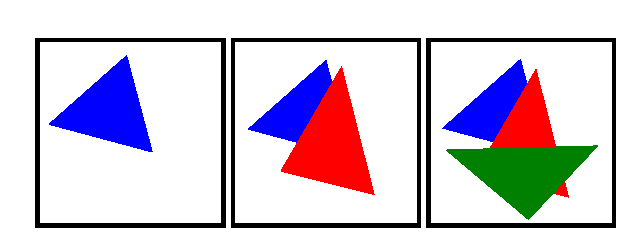
\includegraphics{mccaffreyFigs/default_order.eps}
\end{figure}

On IMR GPUs, this extra bandwidth consumption and fragment work can be limited
by sorting and rendering geometry from front to back.  This is especially
practical for static geometry which can be processed into a spatial data
structure during an asset export step.  An additional heuristic for games is to
render the player character first and the sky-box last.
\cite{Pranckevicius11a}.  

\begin{figure}[h!]
    \caption{By ordering front to back, we know longer shade the covered pixels more than once}
    \centering
        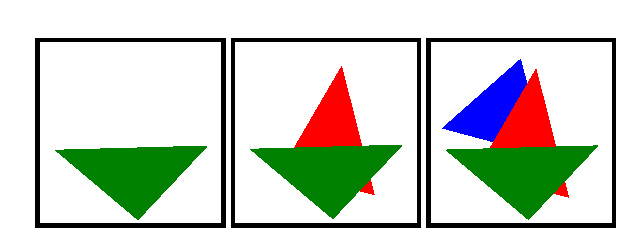
\includegraphics{mccaffreyFigs/order_front_to_back.eps}
\end{figure}

For batches where front-to-back object sorting is not
practical, for example with complicated, interlocking geometry or heavy use of
alpha-testing, a depth prepass can be used to eliminate redundant pixel
calculations, at the cost of repeated vertex shading work, primitive assembly,
and depth-buffer access.

The idea of a depth pre-pass is to bind a trivial fragment shader and render
the scene with color writes disabled.  Depth calculation, testing, and writes
proceed as normal and the final pixel depth is resolved.  The normal
fragment shader is then bound and the scene is re-rendered.  In this manner,
only the final fragments that affect the scene color are rendered.  This only
works for opaque objects.

\begin{figure}[h!]
    \caption{A depth pre-pass resolves ordering in the depth buffer before performing non-trivial fragment shading.}
    \centering
        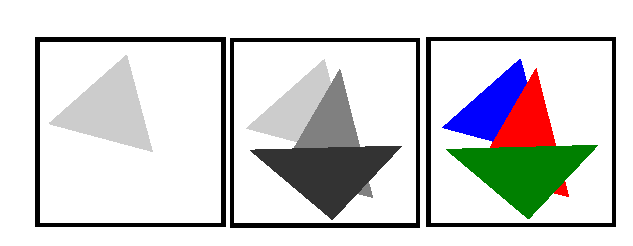
\includegraphics{mccaffreyFigs/depth_pre_pass.eps}
\end{figure}

Even without overdraw, on IMRs heavy amounts of overlapping geometry can still be
expensive because of the depth-buffer reads needed to reject pixels.  Primitive
assembly, rasterization, and the pixel reject rate can also become limiting for
large areas like sky-boxes \cite{Pranckevicius11a}.

One type of effect that can be particular expensive in terms of fragment
shading and framebuffer bandwidth is particle effects rendered via multiple
overlapping quads with blending.  On IMRs, each layer of overlap requires a
read and
 write of the existing framebuffer value.  For all mobile GPUs, each
layers adds additional fragment computation
 and blending.  Some simple
effects
 like a torch flame can be converted into an animated shader, for
example by
 changing a texture offset each frame.  Other effects, like a
candle flame, can
 be done by rendering a mesh of dynamic data, instead of
many overlapping billboarded quads.  This
 reduces overlap and the resultant
blending.  When applicable, using opaque, alpha-tested sprites also eliminates
the cost of blending.

\subsection {Full-Screen Effects}\label{Jon-McCaffrey-Full-Screen-Effects}
Full-screen post-processing effects are a major tool for visual effects in
modern games and graphics applications, and have been an area of innovation in
recent years.   Common applications of full-screen post-processing in games are
motion-blur, depth-of-field, screen-space ambient occlusion, light bloom, color
filtering, and tone-mapping.  Other applications such as photo-editing tools
may use full-screen or large-area effects for composition, blending, warping
and filtering.

Full-screen post-processing is a powerful tool to create effects but it is an
easy way to consume large amounts of bandwidth and fragment processing.  Such
effects should be carefully weighed for their worth, and are prime candidates
for optimization.  

A full-screen pass implies at least a read and write of the framebuffer at full
resolution, which at 16-bit color and a 1024x768 resolution means 188MBps
bandwidth.  Even with tiling architectures, a post-processing pass
means a round-trip to external memory.  One way to optimize these effects is to
remove the extra full-screen pass.  Some post-processing effects such as
color-filtering or tone-mapping that don't require knowledge of neighboring
pixels or feedback from rendering may be merged into the fragment shaders for
the objects themselves.  This may require the use of \textit{uber-shaders} or
shader generation, to allow for natural editing of object fragment shaders
while appending post-processing effects.

If the additional pass cannot be eliminated, then all layered full-screen
post-processing effects can be coalesced into a single additional pass.
Instead of multiple passes that each read the previous result from a texture
and write out a new filtered value, each effect can pass its computed value to
the next effect in the same shader.  This saves redundant round-trips to
framebuffer memory.

\begin{table}[htb]\centering \begin{tabular}{|c||c|c|c|c|c|} 
\hline \small{Device} & \small{clear} & \small{vtx\_lgt} & \small{frg\_lgt} & \small{one\_tap} & \small{five\_tap}  \\ \hline 
\hline \small{Motorola Xoom} & \small{626Mps} & \small{52.4MPps}&  \small{24.08MPps} & \small{26.13MPps\footnotemark[1]} & \small{3.17MPps\footnotemark[1]} \\ 
\hline \small{Motorola Droid X} & \small{3670MPps} & \small{234MPps}& & \small{5.36MPps\footnotemark[1]} & \small{5.7MPps\footnotemark[1]} \\ 
\hline \small{LG Thunderbolt} & \small{305MPps} & \small{48.7MPps}& & \small{30MPps} & \small{20.36MPps} \\ 
\hline \small{Dell Inspiron 520} & \small{1920MPps} & \small{231MPps}& & \small{139MPps} & \small{120MPps} \\ 
\hline \small{Desktop System*} & \small{1380MPps} & \small{2950MPps}& & \small{1730MPps} & \small{1290MPps} \\ 
\hline
\end{tabular} 
 \caption{Performance for different shading and pass
configurations.  All tests used 1024x1024 16-bit offscreen depth and color
buffers as the main framebuffer, with a 32-bit RGBA intermediate color buffer
and 16-bit depth buffer where applicable.  \textit{vtx\_lgt} renders a synthetic
scene with lighting computed per-vertex, a per-pixel texture lookup, and 39200
triangles with 0\% overdraw.  \textit{frg\_lgt} uses the same scene and
calculates the diffuse illumination in the fragment shader.
\textit{five\_tap} and \textit{one\_tap} draw the vertex\_lighting
scene with five- and one- sample full-screen post-processing passes,
respectively.  All units are pixels per second.  Desktop system has an Intel
Core 2 Quad and NVIDIA 8800 GTS.}
 \footnotetext[1] {The DroidX
post-processing scores are low enough that I suspect an implicit render
target-to-texture format conversion must be taking place}
\label{JonMcCaffrey:pass_performance} \end{table}

\index{deferred shading}

One limitation of OpenGL ES 2.0 is poor support for \textit{Multiple Render
Targets (MRT)}, which allow multiple output buffers from a fragment shader.
This makes deferred shading impractical, it relies on separate \textit{geometry
buffers} to store different geometry attributes, but without MRTs, this
requires rendering a full pass of the scene for each.  Even if MRTs
were available however, the additional bandwidth cost of reading and writing
multiple full-screen intermediate buffers make defered shading prohibitively expensive.

\subsection{Off-screen Passes}
\label{Jon-McCaffrey-Off-Screen-Pass}
\index{bloom}
\index{texture filtering}

Similar to full-screen effects are effects requiring off-screen render targets
like environmental reflections, depth-map shadows, and light bloom.

Many of these effects require multiple samples of the off-screen image for a
soft effect.  Since these textures are rendering targets, they probably don't
have full mipmap levels or optimal internal texture layouts for coherent read
access, so eliminating the cost of multiple samples of a large texture is
particularly important One way to optimize off-screen effects that require a
blurred image is to take advantage of texture filtering hardware.  Rather than
rendering a large offscreen image, then taking multiple samples of a fragment
shader, the scene can be rendered into a low-resolution offscreen target and
blurred via texture filtering.

The main fragment shader for the scene can then bind that target as a texture
and read from it with an appropriate texture-filtering mode such as GL\_LINEAR.
The smaller size of the offscreen target makes this strategy particularly
cache-friendly.  This may work well for light bloom and environmental
reflection, for example.  Depending on the effect, an additional Gaussian
blurring pass on the off-screen target may be needed, but these can also be
accelerated with texture filtering and separable kernels as well \cite{Rideout}.

Even when blurring due to texture filtering is not beneficial, reducing
off-screen target resolution is an easy way to reduce the fragment workload
and memory bandwidth without a serious visual impact for effects that only need
low-frequency signals, like environmental reflections.

Whenever moving additional computations from a separate full-screen pass into
the fragment shader of objects in the scene, it is important on non-tiled
architectures to minimize over-draw to avoid wasted work.  One advantage of
full-screen post-processing in a separate pass is that each pixel is computed
exactly once.

\subsection{Shaving Fragment Work}
\label{Jon-McCaffrey-Shaving-Fragment-Work}

One area of optimization with a significant amount of leverage is optimizing
fragment shaders.  Shaders tend to be fairly small and simple, but the sheer
number of fragments and amount of floating-point computation makes non-trivial
fragment shading a major bottleneck on both tiling and IMR GPUs.  Optimizations
here will probably have some effect on visual quality, but it may well be worth
the gain in performance.

For static geometry and lighting, baking most of the illumination into
light-maps saves computation at run-time, and allows the use of more advanced
lighting techniques than would otherwise be affordable \cite{Miller99}
\cite{Unity11}.  Light-map generation and export does require a well-developed
asset pipeline.

Another classic trick to avoid floating-point work and special functions in
fragment shaders is to approximate a complicated function with a look-up
texture \cite{Pranckevicius11b}.  This allows the use of much more elaborate
BDRF's.  This also allows for effects that would be difficult to achieve purely
procedurally \cite{Mitchell07}.  1D look-up textures may be particular
cache-friendly, and with a smooth input parameter should have good locality of
reference.  

However, fragment shaders with multiple texture fetches may already be bound by
texture fetch.  Large amounts of state for each may also limit the maximum
number of in-flight fragments due to register pressure, which affects the
ability of the GPU to hide the latency of texture lookups.

\subsection{Vertex vs. Fragment Work}
\label{Jon-McCaffrey-Vertex-vs-Fragment-Work}

Traditional IMR wisdom states that lifting computations like lighting,
specularity, and normalization from per-fragment to per-vertex and then
interpolating the results can save performance at the cost of image quality,
and this is still true for IMRs.

However, for tilers, this performance wisdom is more dubious because tilers
must perform
 all vertex computations for each tile \cite{Apple11}.  Tilers
are more likely to
 be vertex-bound, and Unity recommends 40k or less vertices
on recent iOS
 devices, which use Imagination Tech SGX GPUs \cite{Unity11}.

This means that heavy vertex shaders, even if they save fragment work, may be
a
 performance drag on tiling architectures.  This is particularly true for
TBDRs since they perform
 little-to-no redundant fragment work.  When working
with IMRs, lifting
 computation from the fragment shader to the vertex shader
is likely a
 performance win, and becoming vertex-bound is less of a concern.

Another consideration to the relationship between vertex and fragment shaders
is that adding too many additional varyings can be a drag on performance, since
they must all be interpolated, and a large amount of per-fragment memory may
limit the number of fragments that can be in-flight at once.  A large number of
varyings may also thrash the post-transform cache, which stores the results of
vertex shading, making vertex processing more expensive.  So thinning the
interface between vertex and fragment shading can be valuable.

Vertex processing is more of a bandwidth drain on tiling architectures, since
the attributes probably are pulled again for each tile, unless they hit in a
pre- or post- transform cache.  To lower this bandwidth, use a lower-precision
buffer format such as \textit{OES\_vertex\_half\_float}.

Interleaved vertex
 data, which interleaves the attributes for each vertex in
the same buffer, is
 also more efficient for attribute fetch, since an entire
vertex can be fetched
 in one linear read \cite{Apple11}.  If there is a
pre-transform vertex
 attribute cache, which stores fetched vertex attributes
and the surrounding
 data, this will make more efficient use of it, since
spatial locality in the
 cache means less data will have to be fetched from
DRAM.

One caveat to interleaving vertex data is if the vertex data is partially
dynamic.  The most common case is when only positions are updated.  A solution
to separate the vertex data into "hot" attributes that are frequently updated
and "cold" ones which are mostly static, and store them in separate buffers.
This avoids inefficient updates to the "hot" attributes because of a large
stride between vertices.

\section{Conclusion}\label{Jon-McCaffrey-Conclusion}

OpenGL ES is a fundamental component of the modern mobile experience, for UI
rendering and composition, \cite{Guy11} and presents a huge market and
potential impact for OpenGL developers.  However, driven by explicit consumer
demand for long battery life and slender devices on one hand, and large,
brilliant displays with perfectly smooth rendering on the other, performance
must be a dominant consideration during development.  The wide range of devices
in the market, differing in age, resolution, and capability, only make
this more difficult.

One important question is if the significant difference in performance
between
 mobile and desktop GPUs will continue to be a dominating
consideration in application development, or if
 it is something that the
steady march of semiconductor process and
 architectural improvements will
soon make irrelevant.  Looking at the projected
 roadmaps for mobile GPU
vendors, the compute power of mobile GPUs should indeed
 climb over the next
few years.  However, other limits, including bandwidth and
 power consumption,
are more fundamental and cannot be conquered as easily.  Desktop and even
laptop systems are less tightly constrained on those dimensions.

The expected workloads of mobile devices are also changing.  Sprite-based games
and 2D workloads are still very important, but several publishers have
produced mobile ports of desktop game engines, and games with console or
desktop levels of rich game worlds and visual quality.  These games raise the
bar for what is considered possible and now expected on mobile systems, and
present challenges in terms of the amount of geometry, assets, and visual
effects they require.  The main strategy to deliver on these promises is a
measured assessment of a platform's capabilities and limitations paired with an
understanding and quantification of the costs of different effects and
rendering techniques.  

While developing a fast and efficient application for mobile devies takes
thought, careful measurement and budgeting, and creative corner-cutting, with a
consciousness to the costs and limitations involved, developers can deliver
beautiful and compelling graphics and an experience users can barely believe is
possible.

\bibliographystyle{akpbib} \bibliography{YourBib}











